%----------------------------------------------------------------------------
\chapter{\saai}
\label{sec:saai}
%----------------------------------------------------------------------------

%----------------------------------------------------------------------------
\section{Program behavior}
\label{sec:progbehavior}
%---------------------------------------------------------------------------- 

Let P be a computer program.

Let $S_{P}^{i}$ be a state of the P program, where at any time P can only be in one state, and at any time P is in one state. A program can be for example represented by its variables' values.

P[S] is the set of states the program can be in.

Let $T_{P}$ be a trajectory of the program. Contains states in certain order to represent an execution.
It can be finite and infinite For example: $T_{P}={S_{P}^{1}, S_{P}^{3}, S_{P}^{5}}$

$T_{P}[S]$ is the set of states the trajectory contains.

So a program behavior can be represented by all the possible trajectories.

\begin{figure} [!ht]
	\centering
	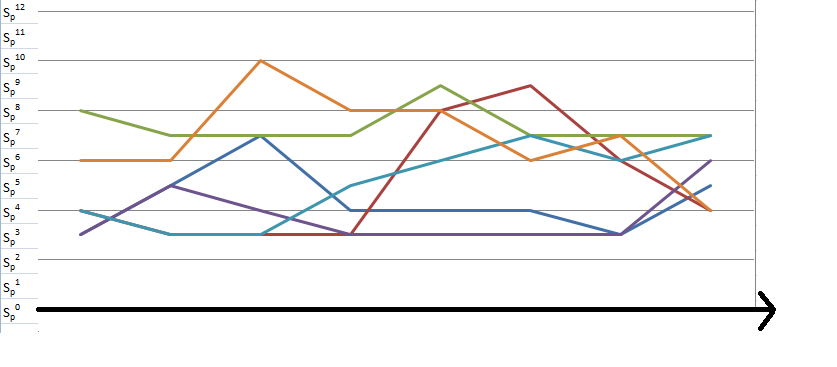
\includegraphics[width=150mm, keepaspectratio]{figures/trajectory1.png}
	\caption{\label{fig:trajectory1}An example trajectories for P}
\end{figure}

For example we want to test that certain states ($S_{P}^{0}$, $S_{P}^{1}$, $S_{P}^{2}$, $S_{P}^{11}$, $S_{P}^{12}$) can be reached at any execution. We have to check every possible trajectory and if none of trajectories contains them than we can say they are unreachable otherwise we can find a counter example. Usually we define error states, what we do not want to reach. We need to prove that none of the trajectories contains error states. 

\begin{figure} [!ht]
	\centering
	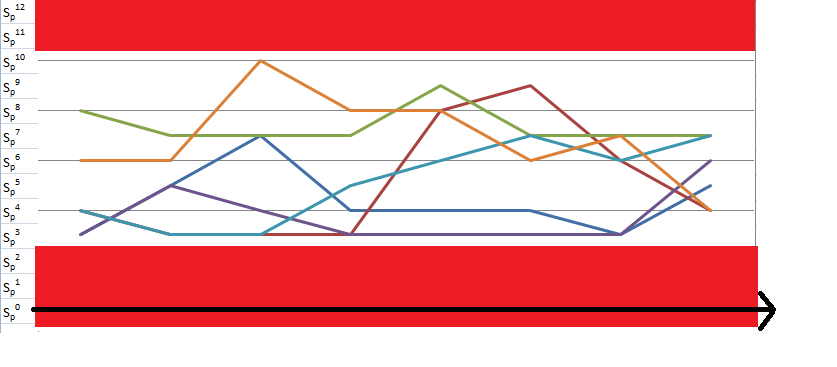
\includegraphics[width=150mm, keepaspectratio]{figures/trajectory2.png}
	\caption{\label{fig:trajectory2}Red shows the error states}
\end{figure}

\begin{figure} [!ht]
	\centering
	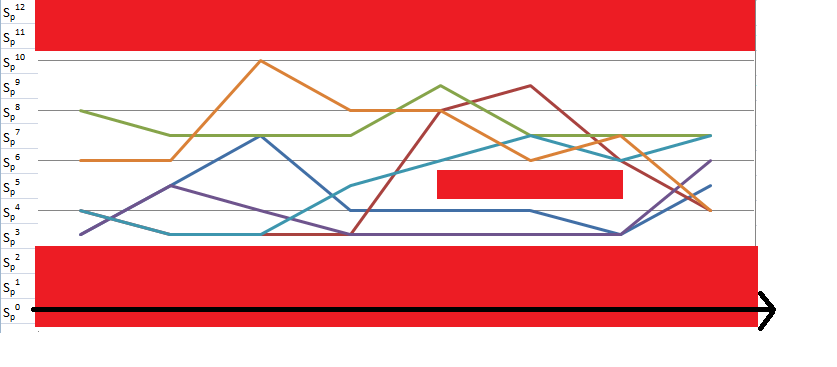
\includegraphics[width=150mm, keepaspectratio]{figures/trajectory3.png}
	\caption{\label{fig:trajectory3}Error state can be time dependent}
\end{figure}

Finding a \hyperref[fig:trajectory4]{counter example} is easier than proving that there is no trajectory which contains error states. 

\begin{figure} [!ht]
	\centering
	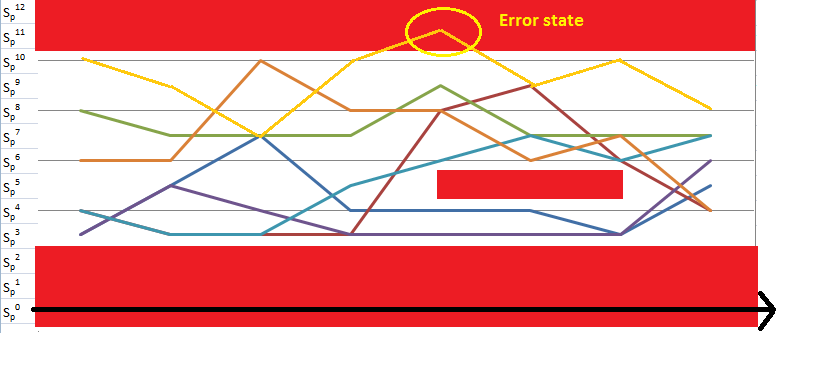
\includegraphics[width=150mm, keepaspectratio]{figures/trajectory4.png}
	\caption{\label{fig:trajectory4}A counter example}
\end{figure}


The problem is that not only there could be many (even infinite) possible trajectories, but some of these can also be infinite. So iterating through all of them is impossible within reasonable time.


%----------------------------------------------------------------------------
\section{Abstraction}
\label{sec:abstraction}
%---------------------------------------------------------------------------- 

The goal of the abstraction is to make it possible to compute in reasonable time that a certain state is reachable or not. Consider what makes it impossible.

(1) P[S] can be infinite
(2) $T_{P}$ can be infinite
(3) there can be infinite number of $T_{P}$-s
  
Abstraction is possible on the states that represents the program. S' is the abstracted state:

$S_{P}^{'1}=S_{P}^{1} \cup S_{P}^{2} \cup S_{P}^{3}$

$S_{P}^{'2}=S_{P}^{4}$

than

$P[S]={S_{P}^{1}, S_{P}^{2}, S_{P}^{3}, S_{P}^{4}}$

$P[S']={S{P}^{'1}, S_{P}^{'2}}$

$T={S_{P}^{1}, S_{P}^{4}, S_{P}^{3}}$

$T'={S_{P}^{'1}, S_{P}^{'2}, S_{P}^{'1}}$

if $S_{P}^{i}$ is error state and $S_{P}^{i} \in S_{P}^{'i}$ than $S_{P}^{'i}$ is error state

Even if the program had infinite states it can now be narrowed to a finite number. For example we define a default S' which contains every state that is not in the other (already abstracted) states. So problem (1) is solved.
 
Fixpoint: Let $T_{P}={S_{P}^{1}, S_{P}^{3}, S_{P}^{5}, ..., *}$ be an infinite trajectory. A fixpoint is the first point, where there are no new states in the trajectory
Formally: (FP=Fixpoint) $min(FP)$ where $T_{P}^{before FP}=$trajectory before Fixpoint, $T_{P}^{after FP}=$trajectory after Fixpoint than $T_{P}^{after FP}[S] \subseteq T_{P}^{before FP}[S]$

We can abstract the infinite trajectory by its sub trajectory before the fix point
Formally  $T_{P}={S_{P}^{1}, S_{P}^{3}, S_{P}^{5}, ..., *}$ and $T'_{P}= T_{P}^{before FP}$ 

By this we do not lose any states that we reached, and if $P[S]$ is finite than $T'_{P}$ will be finite as well. So problem (2) is solved.

Problem (3) is solved, because there are maximum $(longest trajectory)^{|P(S')|}$ trajectories.

Figure \hyperref[fig:trajectory7]{2.5} shows a reachability check where the states abstraction: $P[S']=\{S_{P}^{'error}, S_{P}^{'error!}\}$ where $S_{P}^{'error}=\{S_{P}^{0}$, $S_{P}^{1}$, $S_{P}^{2}$, $S_{P}^{11}$, $S_{P}^{12}\}$ and $S_{P}^{'\not error}=\{S_{P}^{3-10}\}$

 \begin{figure} [!ht]
 	\centering
 	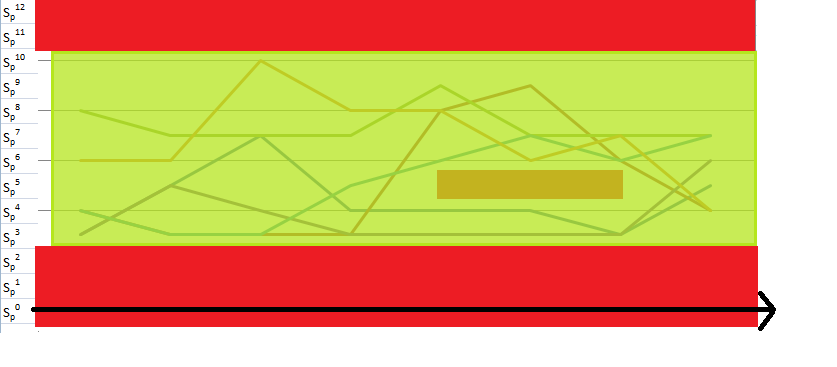
\includegraphics[width=150mm, keepaspectratio]{figures/trajectory7.png}
 	\caption{\label{fig:trajectory7}Reachability check with abstraction}
 \end{figure}


%----------------------------------------------------------------------------
\section{Partition}
\label{sec:partition}
%---------------------------------------------------------------------------- 

Figure \hyperref[fig:trajectory7]{2.5} shows that with the abstraction we proved that $S_{P}^{0}$, $S_{P}^{1}$, $S_{P}^{2}$, $S_{P}^{11}$, $S_{P}^{12}$ states are unreachable, however it can not prove that $S_{P}^{8}$ will not be reached at an erroneous
time. This happens, because during abstraction we lose information.

\begin{theorem}
	It is more important to detect that an error state is reachable than to prove that it is not. This means that, if we say a certain error state is reachable even though it is not then it is tolerable, however if we say it is not reachable even though it is, then it is not tolerable. 	
\end{theorem}
{proof: } The effects of false positive (we said it is reachable, but it was not) will not have any harm, as the programmer can detect that and then he will not take the result into account. However the false negative (we said it is unreachable, but it was) can have severe damage since, the programmer can assume that there is no fault, and if the error occurs especially in safety-critical systems it has serious effects.

One solution for this problem is partition.

 \begin{figure} [!ht]
	\centering
	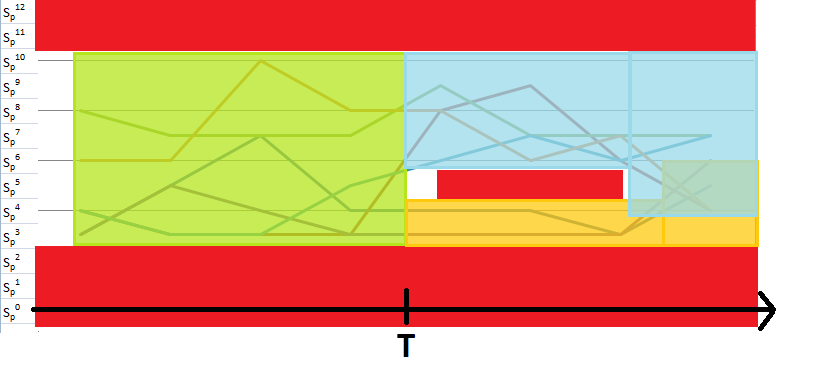
\includegraphics[width=150mm, keepaspectratio]{figures/trajectory8.png}
	\caption{\label{fig:trajectory8}Partition example}
\end{figure}

 In figure \hyperref[fig:trajectory7]{2.6} We start with the same abstraction as in \hyperref[fig:trajectory7]{2.5}, but at T we use partitioning. $P[S']=\{S_{P}^{'error}, S_{P}^{'1} , S_{P}^{'2}\}$ where $S_{P}^{'1}=\{S_{P}^{3}$, $S_{P}^{4}\}$ and $S_{P}^{'2}=\{S_{P}^{6}$, $S_{P}^{7}$, $S_{P}^{8}$, $S_{P}^{9}$, $S_{P}^{10}\}$

%----------------------------------------------------------------------------
\section{Widening}
\label{sec:widening}
%---------------------------------------------------------------------------- 


